\documentclass[a4paper,10pt]{article}

\usepackage{graphicx}
\usepackage{amsfonts}
\usepackage{amssymb}
\usepackage{amsmath}
\usepackage{latexsym}
\usepackage{enumerate}
\usepackage{mdwlist}

%opening
\title{An Exploration of HQSOMS}
\author{Ted Hilk, Joseph Lynch}

\begin{document}

\maketitle

\begin{abstract}

\end{abstract}

\section{Introduction}
\section{Literature Review}
\section{Hypothesis, Plan, and Risks}
\section{System Design and Variables}
HQSOM based networks consist of three basic building blocks: the Self Organizing Map (SOM), the
Recurrent Self Organizing Map (RSOM) and the SOM-RSOM pair.  By composing SOM-RSOM pairs
into larger networks, Hierarchical Quilted Self-Organizing Maps are formed (HQSOM), which can
identify both spatial and temporal clustering in data.  It is important to note that a single
SOM-RSOM pair is still an HQSOM. The general use case for HQSOMs is to cluster data, and then a
supervised learner will actually make the classification because clusters in of themselves do not
provide a classification. The following discussion of SOMs, RSOMs and HQSOMs is based on the work of
Miller and Lommel, and as that is the paper we attempted to replicate the vast majority of this
expositional information can be found in that paper
\cite{HQSOM}
\subsection{SOM}
The basic SOM computional block can either be trained on data or asked to classify data. The SOM is
made up of a $m$x$n$ matrix that maps inputs of dimension $m$ to outputs of dimension $n$.  For
example a SOM designed to take in 3d vectors and output a 5d vector looks like:

\begin{center}
$
\begin{pmatrix}
.3 & .7 & .1  & .14 & .01\\
.3 & .1 & .01 & .16 & .9\\
.3 & .03 & .8 & .7  & .01
\end{pmatrix}
$
\end{center}
Each column is a map unit, and whichever map unit $\bold{w_b}$ is closest to the input $\bold{x}$
is considered the best-matching unit (BMU).  The measure of closeness is usually simply Euclidean
distance, so:
\begin{equation}
 \bold{w_b} = argmin_{w_i} ||\bold{x} - \bold{w_i}||
\end{equation}
 
During the training stage, input vectors are applied to the input and then an
update rule is applied over the entire map space that shifts map units that are nearest to the
input data towards the input data:
\begin{equation} \label{eq:UPDATE}
 \bold{w_{i}}(t+1) = \bold{w_i}(t) + \gamma h_{ib}(t)(\bold{x}(t)-\bold{w_i}(t))
\end{equation}
where gamma is the rate of learning, $h_{ib}$ is the neighborhood function, and $\bold{w_i}$ is the
map unit being modified.  The neighborhood function is defined as a function that is close to zero
for units far away from the BMU.  Traditionally a gaussian is used:
\begin{equation} \label{eq:GAUSSIAN}
 h_{ib}(t) = exp(\frac{-||I_i-I_b||^2}{\mu(t)\sigma^2})
\end{equation}
where $I_i$ indicates the index of the $i$th unit, $\mu(t)$ is a decreasing function of mean
squared error and $\sigma$ is the learning radius.  A SOM therefore has two parameters that need to
be tuned: the learning rate $\gamma$ and the learning radius $\sigma$. For example, two sample unit
maps after an update with $\bold{x}=(.1,.1,.1), \gamma=.2$ and different sigmas would look like:
\begin{figure}[h]
\begin{center}
$
\begin{pmatrix}
0.26 &  0.7 &  0.1 &  0.14  & 0.01 \\
0.26  & 0.1  & 0.01 & 0.16 & 0.9  \\
0.26  & 0.03 & 0.8  & 0.7  & 0.01
\end{pmatrix}$
\caption{$\sigma$ = 1}
\centering
$\begin{pmatrix}
0.26 &  0.607 &  0.1 &  0.139  & 0.01 \\
0.26  & 0.1  & 0.017 & 0.159 & 0.897  \\
0.26  & 0.041 & 0.748  & 0.687  & 0.01
\end{pmatrix}
$
\caption{$\sigma$ = 100}
\end{center}
\end{figure}

During activation, the SOM can return two types of activation vectors:
\begin{enumerate}
\item Discrete: A vector of the correct dimension with the BMU index set to 1 and all others set
to 0.
\item Continous: A vector $A(t)$ defined as the normalized form of a vector constructed as follows:
\begin{equation}
 A_i = \frac{1}{||\bold{x(t)} - \bold{w_i}||^2}
\end{equation}
\end{enumerate}


\subsection{RSOM}
The Recurrent SOM is an extension of the basic SOM that adds a exponential moving average of
differences between observed inputs and units in the map with time-decay parameter $\alpha$ . At
each update the differences are updated and instead of looking for the BMU in map space, the BMU
index is chosen by finding the minimum magnitude recursive difference. Furthermore, instead of
applying $\bold{x}(t)$ directly to the map, the recursive difference for a particular unit is
applied in each unit's update rule and $\bold{x}(t)$ is used to update the recursive difference
matrix:
\begin{equation}
 \bold{y_i}(t+1) = (1-\alpha)\bold{y_i}(t)+\alpha(\bold{x}(t)-\bold{w_i}(t))
\end{equation}
The update rule becomes:
 \begin{equation} \label{eq:RUPDATE}
 \bold{w_{i}}(t+1) = \bold{w_i}(t) + \gamma h_{ib_r}(t)\bold{y(t)}
\end{equation}
where the neighborhood function is computed using the recursive BMU as the BMU index instead of the
map space BMU.  Tuning of $\alpha$ depends on how responsive one wants the RSOM to be: lower values
of $\alpha$ mean a moving average of inputs dominate (long term memory) and higher values of
$\alpha$ (close to 1) mean that recent inputs dominate (short term memory).
\subsection{SOM-RSOM Pair}
The final computational structure is the SOM-RSOM pair.  Recognizing that SOMs are effective at
identifying spatial clustering, and RSOMs are effective at identifying temporal clustering, but
SOMs do zero temporal clustering and RSOMs have degraded spatial clustering, the SOM-RSOM pair is
intended to get the best effect of both.  First the input data is fed into the SOM to get a spatial
representation, and then this representation is fed into the RSOM to do temporal clustering. 
\section{Implementation Process and Results}
Two implementations of SOMs and RSOMs were written, one being as close as possible
to the reference implementation for reproduceability, and the other having a number of slight
changes to improve convergance.  As is to be expected, the reference paper leaves out a
number of implementation details so this is our best approximation.
\subsection{Reference Implementation of SOM and RSOM Units}
Self-Organizing Maps were implemented via a python class with three main methods: a constructor,
an update method that takes a numpy array representing the input vector as well as the learning
parameters (gamma, sigma, etc...) and modifies the internal state of the SOM accordingly, and a
method to request the activation vector for a given input vector. Internally the SOM map was stored
as a $m$x$n$ numpy array where $n$ is the input vector size and $m$ is the size of the map space. 
During an update call, the Best Matching Map Unit (BMU) for any given input vector was determined
using a linear search for the minimum Euclidean distance and then all map units near to the BMU as
well as the BMU were shifted towards the input according to a Gaussian neighborhood function.  The
standard SOM update rule was used as per equation ($\ref{eq:UPDATE}$).
 
A linear search was prefered due to the high dimensionality of the space <CITATION NEEDED>, and a
Gaussian neighborhood function was chosen for reproduceability.  The activation
method returned either a discrete or a continuous representation of the map's activation to a given
input. The discrete representation is defined as above, and the normal representation is given in
equation ($\ref{eq:EUCMETH}$) where $a_i$ represents the $i$th position in the activation vector,
$\bold{w_b}$ is the BMU, $\bold{x}$ is the input vector, and $\bold{w_i}$ represents the $i$th map
unit.
\begin{equation} \label{eq:EUCMETH}
 a_i = \frac{1}{||\bold{w_i}-\bold{x}||}, \bold{a} = \frac{\bold{a}}{||\bold{a}||}
\end{equation}
\\
Recurrent Self-Organizing Maps were simply a subclass of the SOM that use the modified RSOM update
rule as well as storing the recursive difference matrix as a numpy array.  The time decay parameter
($\alpha$) was passed in at every update call.

\subsection{Basic Design of SOM-RSOM Pair and Other Hierarchical Structures}
Since both SOMs and RSOMs are implemented as Python objects, the SOM-RSOM pair simply consisted of
a SOM object and a RSOM object with an update and activation method that takes in an input vector
$\bold{x}$, feeds it into the SOM to get a transformed activation vector $\bold{y}$ and finally
takes that $\bold{y}$ and feeds it into the RSOM to get the final output which is the BMU of the
RSOM.  The only difference between the SOM-RSOM update and activation methods is that the update
method is calling update internally while the activation method is passing along activation
vectors. In the code this SOM-RSOM pair was refered to as a HQSOM because a single SOM-RSOM pair
does indeed form the simplest HQSOM.

Hierarchies were built at first by hard wiring these HQSOM base units together.  However, in order
to facilitate testing of the audio extension, a framework was designed that allowed for any
arbitrary tree HQSOM taking a linear input.  The first level of the tree reads data from the input,
and passes its activation vector to the next layer, which passes its activation vector to the next
layer, etc ...

\subsection{Replication of First Experiment}
The first experiment presented in the paper was a simple example of 3x3 images with 3
pixel horizontal and vertical lines that have been shifted to all possible positions.  This data
set is small enough to be enumerated, and simple enough in concept to use a single SOM-RSOM pair as
the HQSOM network.  We implemented the network as a single HQSOM that had an input size of 9,
internal SOM map size of 18, and internal RSOM map size of 3.  We mapped the 3x3 image grids
to a linear vector of size 9 by iterating through the image left to right and top to bottom.
The mapping used is shown in Figure $\ref{fig:3TestMapping}$.
\begin{figure}[ht]
\begin{center} 
$\begin{pmatrix}
1 & 2 & 3 \\
4 & 5 & 6 \\
7 & 8 & 9 
\end{pmatrix}
\rightarrow
\begin{pmatrix}
1 & 2 & 3 & 4 & 5 & 6 & 7 & 8 & 9 
\end{pmatrix}
$
\end{center} 
\caption{Experiment 1 Image to Vector Mapping}
\label{fig:3TestMapping}
\end{figure} 

The implementation was shown to be correct by two different tests: performance on non-noisy
data, and aggregate performance over many noisy data sets. During training, the HQSOM is exposed to
three blank images, followed by three line images, followed by three blank images where the three
line images alternate between the three horizontal and the three vertical images. An example
training sequence (without noise) is shown in Figure $\ref{fig:3TestData}$.
\begin{figure}[ht]
\begin{center} 
 \includegraphics[scale=.3]{./exp1_dataset.png}
 % exp1_dataset.png: 200x200 pixel, 72dpi, 7.05x7.05 cm, bb=0 0 200 200
\end{center} 
\caption{Experiment 1 Training Sequence}
\label{fig:3TestData}
\end{figure} 
Applying the sequence shown in Figure $\ref{fig:3TestData}$ hundreds of times with parameters
$\gamma_{som} = \gamma_{rsom} = .1, \sigma_{som}=16, \sigma_{rsom}=90,$ and $ \alpha = .1$
trained the HQSOM and clustered the weight vectors in the map units of the SOM and RSOM. Since the
blank images are soley meant to reset the RSOM EMA difference matrix, a method was added to RSOMs
and HQSOMs that allows the difference matrix to be cleared (with a random index selected to have a
value of .01 so that the BMU varies randomly after each reset) and the training steps with blank
images were replaced with a call to this function. After roughly 2500 training samples were shown to
the network, the HQSOM was asked to classify (return the BMU of the top level RSOM) each piece of
data again and as expected all horizontal lines were classified the same, all vertical Lines were
classified the same, and all blank images were classified the same regardless of position.  The
netork had successfully formed an invariant representation of vertical and horizontal lines in a 3x3
field of view.
\\
To test the noise tolerance of the network, gaussian noise with standard deviation .1, .2, .25 and
.3 was applied to the test data, which was then trained on as before and the HQSOM was again asked
to classify samples of noisy vertical and horizontal lines (with different noise from the training
data).  The results of 100 trials with each noise level are summarized in Table
$\ref{table:3TestResults}$.
\begin{center}
  \begin{tabular}{ | c | c | c | }
    \hline
    Noise Std. Deviation & Number Correctly Clustered\\ \hline
    .1 & 99/100 \\ \hline
    .2 & 31/100 \\ \hline
    .25 & 5/100 \\ \hline
    .3 &  4/100\\
    \hline
  \end{tabular}
\label{table:3TestResults}
\end{center}
Clustering ``correctly'' simply means that all vertical lines had the same BMU at the output, all
horizontal lines had the same BMU at the output but different from the vertical lines, and all
blank images had the same BMU at the output but different from either the vertical or horizontal
lines.  For example: $ \begin{pmatrix} 1 & 0 & 0 & 0 & 2 & 2 & 2 \end{pmatrix}$ is a ``correct''
clustering if we apply one blank image, three vertical lines, and three horizontal lines but $
\begin{pmatrix}  2 & 0 & 0 & 0 & 0 & 0 & 0 \end{pmatrix}$ is not. It is worth noting that when fewer
than 2000 training steps were taken the map would often converge to a ``Something vs Nothing'' map
in that the HQSOM would be very goood at clustering lines together and blank images together, but
would not differentiate between the two types of lines.  This makes sense because the alphas 

\subsection{Replication of Second Experiment}
The second experiment presented in the paper aimed to create shift and scale invariant
representations of squares, diamonds, and X shapes in a 7x7 grid.  To replicate this experiment, a
two tiered network was created such that there were 9 low level HQSOMs that each inspected a 3x3
swatch of the 7x7 grid with 1 pixel overlaps on each side which fed a top level HQSOM with a 9
dimensional vector input (composed of the BMUs of each of the bottom level HQSOMs), which in turn
outputed a BMU index representing the cluster an input belongs to. The goal was to find a shift
invariant representation of these shapes by exposing the network to each family of shapes that
are both scaled and then shifted around in a spiral fashion, followed by blanks for 100 steps,
and then the next shape, more blanks, and so on.  The input sequence is shown in Figure
$\ref{fig:7TestData}$.
\begin{figure}
\begin{center}
 \includegraphics[scale=.3]{./exp2_dataset.png}
 % exp2_dataset.png: 813x175 pixel, 72dpi, 28.68x6.17 cm, bb=0 0 813 175
\end{center}
\caption{Experiment 1 Training Sequence}
\label{fig:7TestData}
\end{figure} 

The paper claims upward of 95\% clustering, but we were unable to even achieve a four
classifier using the specified parameters in the paper as per Figure $\ref{fig:PAPERSPECS}$. 
\begin{figure}[ht] 
 \begin{center}
  \begin{tabular}{ | l | c | c | c | c | }
    \hline
    & $\gamma$ & $\alpha$ & $\sigma$ & Map Size\\ \hline
    Layer 1 SOMs  & .1   & 1   & 4  & 65\\ \hline
    Layer 1 RSOMs & .01  & .1  & 10 & 17\\ \hline
    Layer 2 SOMs  & .1   & 1   & 2  & 513\\ \hline
    Layer 2 RSOMs &  .001 & .01 & 50 & 17 \\
    \hline
  \end{tabular}
\caption{Experiment 2 Parameters}
\label{fig:PAPERSPECS}
\end{center}
\
\end{figure}

The best
run of our HQSOM yielded the following final distribution where the final distribution is simply the
number of test images classified as that BMU divided by the total number of test images for a given
data set.

\begin{center}
\small
\begin{verbatim}
################################################################################
Data Set: BLANK
Most Frequently Classified As (MODE): 4
Full Distribution over Final RSOM Map Space:
[ 0.  0.  0.  0.  1.  0.  0.  0.  0.  0.  0.  0.  0.  0.  0.  0.  0.]
################################################################################
Data Set: SQUARE
Most Frequently Classified As (MODE): 3
Full Distribution over Final RSOM Map Space:
[ 0.          0.08571429  0.17142857  0.45714286  0.28571429  0.          0.
  0.          0.          0.          0.          0.          0.          0.
  0.          0.          0.        ]
################################################################################
Data Set: DIAMOND
Most Frequently Classified As (MODE): 2
Full Distribution over Final RSOM Map Space:
[ 0.          0.14285714  0.77142857  0.08571429  0.          0.          0.
  0.          0.          0.          0.          0.          0.          0.
  0.          0.          0.        ]
################################################################################
Data Set: X
Most Frequently Classified As (MODE): 2
Full Distribution over Final RSOM Map Space:
[ 0.          0.          0.97142857  0.02857143  0.          0.          0.
  0.          0.          0.          0.          0.          0.          0.
  0.          0.          0.        ]

\end{verbatim} 
\end{center}

While there is certainly convergance, it is not 95\%.  Due to the fact that runs of this particular
simulation took well over 9 hours, we were only able to test about 10 different
parameter combinations, none of which yielded a better result then the one supplied above.  It
appeared that the HQSOM was not using the full breadth of the RSOM map space in any of the HQSOM
units, which was likely because the activation vectors passed up were incorrect.  This was likely
the cause because the implementation of continuous activation vectors was deduced but not taken
directly from the paper due to unclear explanation in the paper of how they passed activation
vectors.  It was also noticed that the networks fequently converged to certain states very quickly
and then never moved from that state.  The lack of a good activation vector and fast convergance
led us to the following innovations:
\begin{enumerate}
\item A regularized activation vector based on the Mean Squared Error of the BMU vector.
\item The notion of an adaptive $\gamma$.
\item The use of a Mexican Hat neighborhood function (second derivative of Gaussian) instead of a
Gaussian neighborhood function.
\end{enumerate}
 
\subsection{Changes to Algorithm and Relative Performance}
Having completed the implementation of the paper's networks as far as deemed feasible, the three
innovations previously mentioned were implemented in code and tested to compare relative
performance. In all cases our implementation proved to be superior, especially when we began
testing our Audio extension.
\\
\\
We began by implementing the new activation vector.  Since the adaptive $sigma$ function was based
on minimizing the mean-squared error (MSE) of the BMU and input vector, we believed that it would
also be a good metric to measure activation by.  This lead to the definition in equation
($\ref{eq:MSEMETH}$) where the vector parameters are the same as in equation ($\ref{eq:EUCMETH}$)
except that now $MSE(\bold{x},\bold{y})$ indicates the mean squared error between vectors
$\bold{x}$ and $\bold{y}$.
\begin{equation} \label{eq:MSEMETH}
 a_i = \frac{MSE(\bold{w_b}, \bold{x})^3}{MSE(\bold{w_i},\bold{x})^3}
\end{equation}
The cube was so that the distribution in the vector would be more concentrated on the BMU's index.
\\
\\
Next we implemented the adaptive $\gamma$.  During testing, the MSE between the input and BMU would
often spike due to a training example that had never been seen before, which would cause $\sigma$ to
spike, which would in turn pull the entire map space drastically towards the new training example. 
This led to things like oscillations between two clusters while entirely losing a third or fourth
possible clustering.  To remedy this problem, we kept an exponential moving average of MSE in the
SOMs of each HQSOM unit and whenever the MSE spiked by more than an order of magnitude, we made
$\gamma$ equal to some high fraction (in our case .6) just for the update of the BMU weight.  This
meant that a single map unit was pulled into the new cluster, becoming the semi-permanent BMU for
all new training data that fell in that cluster.
\\
\\
Lastly we replaced equation $\ref{eq:GAUSSIAN}$ with equation $\ref{eq:MEXICANHAT}$.
\begin{equation}\label{eq:MEXICANHAT}
 h_{ib}(t) = (1-\frac{||I_i-I_b||^2}{\sigma^2})*exp(\frac{-||I_i-I_b||^2}{\mu(t)\sigma^2})
\end{equation}
The advantage of this function is that it pushes away map units that are near to the input,
but far enough away to be considered not matching.  This helps deal with the pre-matrure convergance
noticed during testing. The negative aspect of this function is that the $\sigma$ parameter has to
be chosed very carefully so as to prevent uniform distributions from forming.
\\
\\
With our improvements in place, we re-ran the noise tolerance test from Experiment 1 and the large
network test from Experiment 2.  The results for the noise tolerance test over 100 runs is
summarized in table $\ref{fig:3BetterTestResults}$.
\begin{figure}[ht]
\begin{center}
  \begin{tabular}{ | c | c | c | c | }
    \hline
    Noise Std. Deviation & Paper Implementation& Our Implementation \\ \hline
    .1 & 99/100 & 100/100 \\ \hline
    .2 & 31/100 & 73/100\\ \hline
    .25 & 5/100 & 39/100\\ \hline
    .3 &  4/100 & 12/100\\
    \hline
  \end{tabular}
\end{center}
\caption{Experiment 1 Test with Noisy Data: Clustering Results }
\label{fig:3BetterTestResults}
\end{figure}

Clearly our implementation represents a significant improvement in the face of noisy data.  This is
most likely due to the fact that we better allow for late cycle plasticity and are therefore able
to compensate for early noisy examples with later less noisy examples.
\\
\\
Once again the second experiment proved challenging.  We were unable to get any better results with
the parameters provided in the paper, but by using the following network parameters, we were able
to get a nearly equivalent result with far fewer cpu cycles:
\begin{center}
  \begin{tabular}{ | l | c | c | c | c | }
    \hline
    & $\gamma$ & $\alpha$ & $\sigma$ & Map Size\\ \hline
    Layer 1 SOMs  & .1   & 1   & $\sqrt{20}$  & 40\\ \hline
    Layer 1 RSOMs & .01  & .1  & $\sqrt{150}$ & 25\\ \hline
    Layer 2 SOMs  & .1   & 1   & $\sqrt{15}$  & 150\\ \hline
    Layer 2 RSOMs &  .05 & .02 & 50 & 7 \\
    \hline
  \end{tabular}
\end{center}
\begin{center}
 \small

\begin{verbatim}
################################################################################
Data Set: BLANK
Most Frequently Classified As (MODE): 2
Full Distribution over Final RSOM Map Space:
[ 0.  0.  1.  0.  0.  0.  0.]
################################################################################
Data Set: SQUARE
Most Frequently Classified As (MODE): 0
Full Distribution over Final RSOM Map Space:
[ 0.343  0.     0.314  0.171  0.143  0.029  0.   ]
################################################################################
Data Set: DIAMOND
Most Frequently Classified As (MODE): 2
Full Distribution over Final RSOM Map Space:
[ 0.     0.     0.457  0.171  0.029  0.029  0.314]
################################################################################
Data Set: X
Most Frequently Classified As (MODE): 6
Full Distribution over Final RSOM Map Space:
[ 0.     0.     0.2    0.2    0.2    0.057  0.343]
SUCCESS
\end{verbatim}
\end{center}

When run with the same network, the reference implementation only produced two main statistical
clusters.  Once again, our implementation seemed superior.  


\subsection{Extension into Audio}
The final stage of our project was extending our framework into audio classification.  The goal was
to be able to give a HQSOM spectrograms, and have the network cluster like genres together. 
The first step of implementation was to build a generic framework that would allow for any arbitrary
tree type network to be constructed without hard-wiring the HQSOMs together.  Then, a test
framework was created that allowed us to take 15 second snippets of songs, compute FFTs over windows
that lasted $\frac{1}{10}$ of a second for each song, and puncture the FFTs such that we reduced the
input space to a 128 dimension vector.  At the end of data processing we had the six FFTs shown in
Figure $\ref{fig:FFTS}$. The data were derived from the following songs:
\begin{enumerate}
 \item Techno (Training) - Rudenko - Everybody
 \item Techno (Testing) - Kid Cudi - Day and Night
 \item Rock (Training) - Red Hot Chili Peppers, Californication
 \item Rock (Testing) - Red Hot Chili Peppers, By the Way
 \item Classical(Training) - Unknown Orchestra Conducted By George Winston - Carol Of The Bells
 \item Classical(Testing) - Beethoven - Symphony No. 9
\end{enumerate}
The ``Training'' tag indicates that the network was exposed to sequential samples of that song's
FFTs in entirety, and then shown random 1 second clips from the Spectrogram in rotation with the
other Training songs. ``Testing'' songs were never exposed to the network during the training
phase, but during the classification stage the HQSOM was asked to classify them. Unfortunately,
every prototype network we tried with the reference SOM-RSOM implementation converged to a constant
BMU within one or two training cycles. A network was built that consisted of two base SOM-RSOM
nodes that take in 64 inputs each (half of the 128) and each output a BMU to a second SOM-RSOM,
which then output their BMUs to a combined 2d vector which is used as the input to a final SOM-RSOM
node which outputs the classification BMU (See the attached code for exact parameter details).  When
we used this network in conjunction with our improvements we were able to get the following results:
\begin{center}
\begin{verbatim}
################################################################################
Results for Techno
Final Distribution Over Map Space
[ 0.265  0.349  0.     0.386  0.   ]
MODE: 3
################################################################################
Results for TechnoTEST
Final Distribution Over Map Space
[ 0.287  0.275  0.     0.438  0.   ]
MODE: 3
################################################################################
Results for Classical
Final Distribution Over Map Space
[ 0.526  0.154  0.     0.321  0.   ]
MODE: 0
################################################################################
Results for ClassicalTEST
Final Distribution Over Map Space
[ 0.49   0.202  0.     0.308  0.   ]
MODE: 0
################################################################################
Results for Rock
Final Distribution Over Map Space
[ 0.434  0.554  0.     0.012  0.   ]
MODE: 1
################################################################################
Results for RockTEST
Final Distribution Over Map Space
[ 0.266  0.734  0.     0.     0.   ]
MODE: 1
\end{verbatim}
\end{center}

This is the result after cycling through each training song in entirety, followed by three random 1
second window exposures for each song, making sure to clear the HQSOM's difference matrix when
switching songs.  The above is not a perfect clustering of data, but it does show that the network
formed a weak invariant representation of different genres, after only a single training cycle.  It
is important to note that it took quite a bit of tweaking of parameters to get the above results,
but it is a perfectly fine proof of concept.

\begin{figure}
\begin{center}
  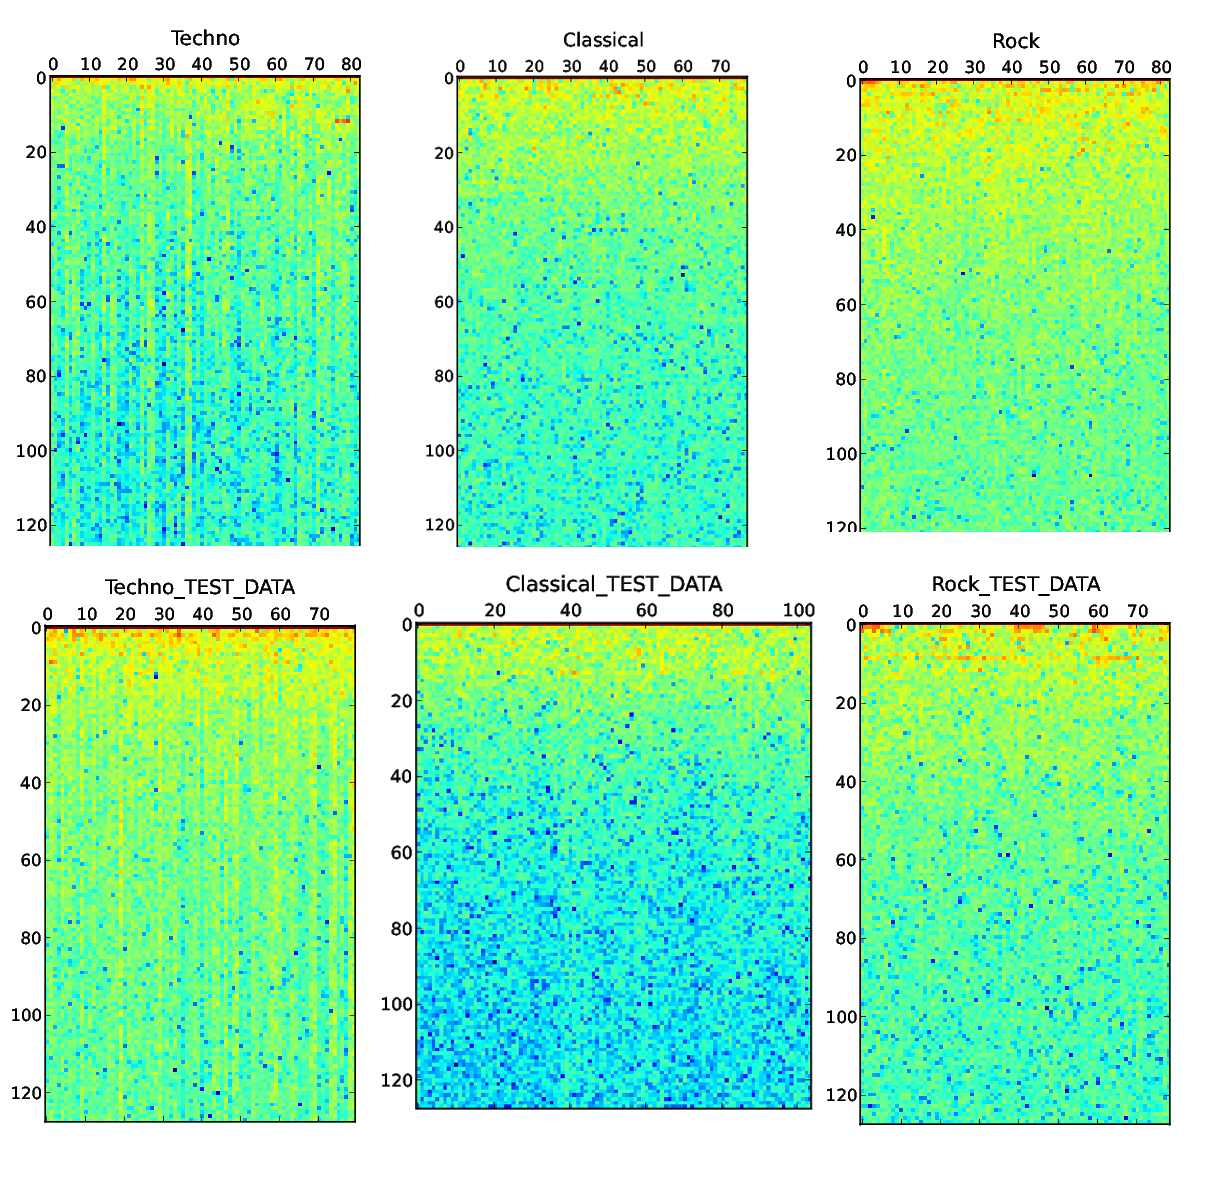
\includegraphics[scale=.2]{./all_ffts.png}
 % exp2_dataset.png: 813x175 pixel, 72dpi, 28.68x6.17 cm, bb=0 0 813 175
\end{center}
\caption{Experiment 1 Training Sequence}
\label{fig:FFTS}
\end{figure} 




\subsection{Problems}
\section{Discussion and Conclusions}
\section{References}

\begin{thebibliography}{}
\bibitem{HQSOM} J. W. Miller and P. H. Lommel. \textsc{Biomimetic sensory abstraction using
hierarchical quilted self-organizing maps}. The Charles Stark Draper Laboratory, Inc.
555 Technology Square, Cambridge, MA 02139-3563, USA. 2006.
\end{thebibliography}

\end{document}
